\documentclass[12pt, a4paper]{article}

% \cite{weiss} pentru cartea din care citim
% \cite{prakken} este referința [36]
% \cite{aif} este referinta [11] (Towards an Argument Interchange Format)
% \cite{modgil} este referința [30]

\title{Argumentation among Agents:\\Review and Commentary}
\author{Grigore Costin-Teodor\quad Radu Ștefan-Octavian\\Vasiliu Florin\quad Vintilă Eduard}
\date{}


\usepackage{tikz}
\usetikzlibrary{arrows.meta}

\usepackage{amsfonts}
\usepackage{hyperref}

% Utilizează biblatex pentru referințe bibliografice
\usepackage[
maxbibnames=50,
sorting=nty
]{biblatex}

% Fișierul cu bibliografia
\addbibresource{bibliography.bib}

\usepackage{mathtools} % pentru sageti cu scris peste

\newcommand{\df}{\ensuremath{\rightharpoonup}}
\newtheorem{Def}{Definition}[subsection]
\newtheorem{Ex}{Example}[subsection]
\newtheorem{Claim}{Claim}


\begin{document}

\maketitle

\section{Introduction}

The present essay is, essentially, a summary of Iyad Rahwan's \emph{Argumentation among Agents}, which appears as Chapter~5 in~\cite{weiss}. Where feasible, we have tried to phrase the given definitions more clearly, as well as to provide our own examples. The material is covered in the same order as in the given reference.

\section{Several notions of ``argumentation''}

Before passing on to the ``multiagent'' half of the title, the author exhibits three formalizations of the ``argumentation'' concept, all pre-existent in the literature. By employing mathematical descriptions, these differ from the philosopher's viewpoint, which is expressed informally: an argument consists of the giving of claims in favor or against a statement that is open for debate.

\subsection{Prakken's framework}

Since this first framework is stated for reference, but used infrequently, we take the liberty of presenting a trimmed down version, that nevertheless contains all the components which the book elaborates upon.

As can be seen more clearly in Prakken's original article~\cite{prakken}, his ``argumentation system'' is very similar to common logics---the major difference being the existence of two distinct kinds of inference rules: \emph{strict} and \emph{defeasible}. (Note that ``defeasible'' means ``open to objection''.)

Concretely, we take an \emph{argumentation system} to be a tuple \( (\mathcal{L}, \mathit{cont}, S, D) \), where $\mathcal{L}$ is a ``logical language'' (not much more is given about it, except that it should contain negation), $\mathit{cont}$ is the so-called \emph{contrariness} function, and $S, D$ are, respectively, the strict and defeasible sets of inference rules. With respect to the $cont$ function, we note that it takes a member of $\mathcal{L}$ (henceforth referred to as a \emph{formula}), and returns a set of formulas. Its purpose is to generalize ordinary negation. To show how, we extract again from Prakken~\cite[page 97]{prakken}: if \( \varphi \in \mathit{cont}(\psi) \), then
\begin{itemize}
\item If \( \psi \not\in \mathit{cont}(\varphi) \), then $\varphi$ is a \emph{contrary} of $\psi$;
\item If \( \psi \in \mathit{cont}(\varphi) \), then $\varphi$ and $\psi$ are \emph{contradictory}.
\end{itemize}
Moreover, it is assumed that \( \neg\varphi \in \mathit{cont}(\varphi) \) and \( \varphi \in \mathit{cont}(\neg\varphi) \). Thus, a formula and its negation are contradictory, but neither is merely a contrary of the other.

We conclude this section by hinting at the definition of an \emph{argument}. Note that inference rules transform a set of premises into a single conclusion (all of these are formulas). In writing, the distinction between strict and defeasible rules is given by the shape of the arrow symbol that is used. For instance, \( p, q \rightarrow r \) indicates strictness: $r$ surely follows from $p$ and $q$. Defeasibility is illustrated thus: \( u \Rightarrow v \), which informally means ``$v$ presumably follows from $u$''. Starting from a set of formulas known as the \emph{knowledge base}, an argument is then defined inductively to be one of the following:
\begin{itemize}
\item A member of the knowledge base.
\item A tuple consisting of some arguments and a ``conclusion'' formula, written as \( A_{1},\ldots,A_{n} \rightarrow \varphi \), such that $\varphi$ follows via a strict rule from the conclusions of $A_{1},\ldots,A_{n}$.
\item Likewise for a defeasible rule.
\end{itemize}
The complete framework also contains a partial order on the defeasible rules, indicating their ``preferability''. Using it, arguments may be compared. (In passing we note that Prakken's paper uses the baffling term ``partial preorder''.)

\subsection{Dung's model}

We now skip directly to the argumentation model that is to be used most frequently in upcoming sections. Observe that Prakken's framework deals with the internal structure of arguments---their construction. The current model, due to Dung, considers arguments as completed entities. Following him, from now on, unless stated otherwise, an \emph{argumentation framework} will be a finite directed graph, whose nodes are called ``arguments''. The adjacency relation is pronounced ``defeats''. Note that, as usual, this directed graph is a pair $(\mathcal{A}, \df)$, where $\mathcal{A}$ is a finite set and $\df$ is a binary relation on $\mathcal{A}$. Hence, $p \df q$ means ``$p$ defeats $q$''. (Notationally, we have deviated from the author only in using Latin letters for variables ranging over arguments.) Henceforth, the discussion is conducted with respect to a fixed argumentation framework.

Our next task is to examine what makes an argument acceptable. In stating the following definitions, we adopt a primarily non-symbolic style of exposition, which facilitates understanding of the motivation behind them. As a further contribution, for illustration, we use our own example of an argumentation framework, visible in Figure~\ref{af}. We shall refer to it as ``the running example''.
\begin{figure}
\centering
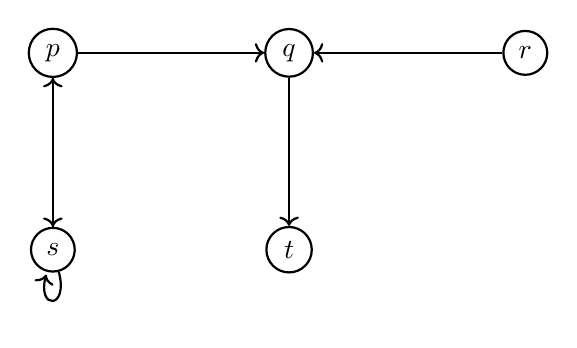
\begin{tikzpicture}
\tikzstyle{vertex} = [circle, draw = black, thick]
\tikzstyle{edge} = [->, thick]
\node[vertex] (p) at (0, 0) {$p$};
\node[vertex] (q) at (3, 0) {$q$};
\node[vertex] (r) at (6, 0) {$r$};
\node[vertex] (s) at (0, -2.5) {$s$};
\node[vertex] (t) at (3, -2.5) {$t$};
\draw[edge] (p)--(q);
\draw[edge] (p)--(s);
\draw[edge] (q)--(t);
\draw[edge] (r)--(q);
\draw[edge] (s)--(p);
\path (s) edge [loop below, thick] node {} (s);
\end{tikzpicture}
\caption{The running example.} \label{af}
\end{figure}
\begin{Def}[$+$ and $-$ operators]
For a set $S$ of arguments, $S^{+}$ is the set of all arguments defeated by some member of $S$. For argument $p$, $p^{-}$ is the set of all arguments which defeat $p$.
\end{Def}
For instance, in the running example, $\{ p, q \}^{+} = \{ q, s, t \}$ and $s^{-} = \{ p, s \}$.
\begin{Def}[conflict-freeness, defending]
A set $S$ of arguments is \emph{conflict-free} if no argument in $S$ defeats another also in $S$. Graph-wise, this means that there is no edge between two nodes in $S$. Also, we say $S$ \emph{defends} $p$ if every argument which defeats $p$ is defeated by $S$ (i.e., is in $S^{+}$).
\end{Def}
In the running example, the sets $\{ p, t \}$ and $\{ r, t \}$ are conflict-free. It may also be said that $\{ p, t \}$ defends $t$, since $t$ is only defeated by $q$, and $p$ defeats $q$.
\begin{Def}[characteristic function]
The \emph{characteristic function}, labelled $\mathcal{F}$, takes a set $S$ of arguments and returns the set of arguments defended by $S$.
\end{Def}
In the running example, $\mathcal{F}(\{ p, q, r \}) = \{ r, t \}$ and $\mathcal{F}(\{ r, t \}) = \{ r, t \}$.

From this point on, we believe brevity surpasses transparency as a concern, so we revert to more symbolism.
\begin{Def}[admissibility, complete extension]
Let $S$ be a conflict-free set. $S$ is \emph{admissible} if $S \subseteq \mathcal{F}(S)$. (This latter condition means that $S$ defends all its members.) If $S = \mathcal{F}(S)$ (i.e., $S$ defends its members and nothing else), then $S$ is a \emph{complete extension}.
\end{Def}
By the previous remarks, it may be seen that $\{ r, t \}$ is a complete extension.

Finally, we exhibit what the author calls ``an equivalent characterization of complete extensions'' (we shall supply a proof for one side of this equivalence---such a proof is not present in the chapter).
\begin{Def}[labelling]
\sloppy A labelling is a function $L$ from $\mathcal{A}$ to $ \{ \mathtt{in}, \mathtt{out}, \mathtt{undec} \} $. It satisfies the following properties:
\begin{itemize}
\item $L(p) = \mathtt{in}$\quad iff all attackers of $p$ are $\mathtt{out}$ (under $L$),
\item $L(p) = \mathtt{out}$\quad iff some attacker of $p$ is $\mathtt{in}$,
\item $L(p) = \mathtt{undec}$\quad otherwise.
\end{itemize}
\end{Def}
We have used the expression ``attacker of $p$'' to designate a node which defeats $p$. The term seems more convenient in speech, although less proper than the author's ``defeater''.

It is claimed that, given a valid labelling, the nodes marked ``\texttt{in}'' constitute a complete extension.\\

\noindent\textbf{Proof of claim}\quad Let $S$ be the set of nodes labelled ``\texttt{in}''. First, we show that $S$ is conflict-free. This can be seen immediately by the first condition imposed on a labelling: all attackers of members of $S$ are \texttt{out}, and hence not in $S$.

Secondly, we prove the two necessary inclusions:
\begin{itemize}
\item $S \subseteq \mathcal{F}(S)$.\quad Let $p \in S$. We have to show that $p$ is defended by $S$. Let $q$ be an attacker of $p$. By the properties of a labelling, $q$ is \texttt{out}, and so it has an attacker that is \texttt{in}, i.e., $\in S$.
\item $\mathcal{F}(S) \subseteq S$.\quad Assume $p \not\in S$. If $p$ is \texttt{out}, then it has an attacker in $S$, which certainly cannot be defeated by $S$, since $S$ is conflict-free. Hence, $p \not\in \mathcal{F}(S)$. If $p$ is \texttt{undec}, then it has an attacker $q$ that is \texttt{undec} also. This $q$ cannot be attacked by a member of $S$ since that would make it \texttt{out}. Thus again $p \not\in \mathcal{F}(S)$.
\end{itemize}

Indeed, for the running example, it may be checked that a function which assigns \texttt{in} to $r, t$, \texttt{out} to $q$, and \texttt{undec} to $p, s$, is a labelling.

Certain other kinds of extension (besides complete) are discussed. We do not delve into their details here. What is of interest is the next, and final, definition. It introduces the degrees of acceptability of an argument---their statement being the objective of this section.

\begin{Def}
An argument $p$ is:
\begin{itemize}
\item \emph{skeptically accepted} iff $p$ belongs to every extension,
\item \emph{credulously accepted} iff $p$ belongs to some extension,
\item \emph{rejected} iff $p$ doesn't belong to any extension.
\end{itemize}
\end{Def}

\newpage
% ===================================================



% =================Edi's work========================
\section{Argumentation Protocols}
In the previous section, we have presented two possible models for formalizing the idea of argumentation: Prakken's framework and Dung's model. We find that both of them manage to  capture the intuition behind the essence of an argument reasonably well. However, we shall see that the author focuses on the latter model to present a mechanism by which two agents can participate in a \emph{dispute} where they can state and attack each other's arguments, much as in a real world debate.

As such, this section focuses on formalizing these "argumentation games" and also a set of constraints used in regulating the whole argumentation process in order to prevent situations where an agent might contradict himself, for example. These rules are called argumentation protocols and Dung's model proves to be particularly effective for them, since we do not have to deal with the internal structure of the arguments.

\subsection{Argumentation Games}
We begin by fixing the environment in which the argumentation process takes place. Essentially, we want to model a game where one player proposes an initial argument, after which both players take turns in counter-attacking the counterpart's last argument by specifying one which defeats it. The game shall be considered to be won by the player who lastly put forward an argument which could not be defeated by its opponent.

The author refers to Modgil and Caminada's work \cite{modgil} for describing such a game, where the two players are defined as PRO (as in, the proponent which states the initial argument) and OPP (the opponent, which begins by counter-attacking the argument proposed by PRO). We provide the following formal definition of what represents a "dispute", a notion which captures the moves done by the players to attack the counterpart's arguments and is merely stated in natural language by the author:

\begin{Def}[dispute]
	Given an argumentation framework $(\mathcal{A}, \df)$, a dispute is a sequence $(a_{k})_{k \in \mathbb{N}}$ (possibly infinite) of arguments from $\mathcal{A}$ where the following property holds: $\forall i \in \mathbb{N^*},  a_{i} \df a_{i-1}$ (i.e. every argument in the sequence defeats its preceding argument).
\end{Def}

From the above definition, we can thus consider that even indexed elements in the sequence (starting from $a_0$) are the arguments stated by the PRO player, and the odd ones by the OPP player. We can additionally define what it means to win a dispute:

\begin{Def}[winning of a dispute]
	A finite dispute $d = (a_{k})_{k=0}^{n}$, where $n \in \mathbb{N}$ is the index of the last argument in $d$, is said to be won by the PRO player iff $n$ is even and no argument from $\mathcal{A}$ can defeat $a_n$. Consequently, the dispute $d$ is considered to be won by the OPP player iff $n$ is odd and no argument from $\mathcal{A}$ can defeat $a_n$ .
\end{Def}

This corresponds to the the established semantics by which a player wins only if its counterpart player cannot defeat the last argument that has been stated. Notice how the sequence of arguments must be finite in order to establish a winner - if the sequence would have been infinite, hence unbounded, we could not pronounce a winner since there would not exist a last argument in the dispute.

We observe that a player could potentially counter-attack its counterpart player with any argument whatsoever that defeats the last move. This leads to multiple disputes based on the defeating argument chosen by the player, which can be conveniently modeled as a dispute tree, as shown by the author. Such a tree can be constructed with the initial argument stated by the PRO player as a root node and child nodes as arguments which defeat the parent node. As such, all paths from root to leaf will represent all possible disputes for a given starting argument. We propose the following definition for a dispute tree, inspired by \cite{modgil}:

\begin{Def}[dispute trees]
	Given an argumentation framework\\ $(\mathcal{A}, \df)$ and an argument $p$ in $\mathcal{A}$, a dispute tree induced by $p$ is a tree $T$ rooted in $p$, where each node represents an argument from $\mathcal{A}$ and for all arguments $x, y$ in $\mathcal{A}$, $x$ is a child of $y$ in $T$ iff $x$ defeats $y$.
\end{Def}

Notice how each level of a dispute tree corresponds to arguments stated by either the PRO or the OPP player. If we count the levels of the tree starting from 0, then each even-numbered level marks arguments moved by the PRO player, and consequently odd-numbered levels represent arguments from the OPP player. As such, we can now consider a \emph{dispute} merely a path in such a tree, and we shall see that further definitions and theorems stated by the author use this assumption.


However, since we have seen that disputes can potentially represent infinite sequences of arguments, this can lead, of course, to never-ending paths in a dispute tree where we cannot therefore pronounce a winner (we consider that a tree is finite if all of its paths are of finite length). Fortunately, we can avoid such situations by imposing a set of constraints by which a player cannot simply choose any argument that defeats its opponent's. One possible rule could describe that a player cannot state an argument which defeats any of its previous arguments in the dispute, for example (in other words, the set of arguments uttered by the player is \emph{conflict-free}). By imposing such rules, we can capture various semantics of an argumentation game, such as a player cannot contradict himself, as is the case with the example rule that we have given. This is exactly the intuition behind an argumentation protocol, a notion which the author uses to introduce constraints that no longer allow infinite decision trees, through the definition of a protocol called $G$.

\begin{Def}[dispute tree under protocol G]\label{protG}
	Given a dispute tree $T$, we consider $T$ to be under protocol G iff for any arbitrary dispute $d$ in $T$ and for any pair of arguments $x$, $y$ stated by PRO in $d$, $x$ is different than $y$.
\end{Def}

A dispute tree $T$ under a protocol $G$ essentially ensures that PRO does not state an argument which has been previously uttered by him. It is claimed by the author that the following holds:

\begin{Claim}
	If $T$ is a dispute tree under protocol $G$, then $T$ is finite.
\end{Claim}


\noindent\textbf{Proof of claim}\quad Let $T$ be a dispute tree under protocol G, induced by an argument $p$ from an argumentation framework $(\mathcal{A}, \df)$, where $\mathcal{A}$ is a finite set of arguments with $n \in \mathbb{N^*}$ such that $card(\mathcal{A}) = n$. Let $d = (a_{k})_{k \in \mathbb{N}}$ be a dispute in $T$ of length of at least $2n$ arguments (we do not consider the other disputes, since we know they are of finite length).

%, and $m \in\mathbb{N}$ such that $m = 2n - 1$
We shall prove that $d$ is of finite length; more specifically, exactly of length $2n$. We consider the argument $a_{2n - 1}$ from our sequence $d$. Without loss of generality, we establish $PRO_{2n-1}(d) = (a_{2k})_{k=0}^{n-1}$ to be the arguments uttered by PRO until argument $a_{2n - 1}$ (stated by OPP) from dispute $d$. By definition \ref{protG}, we have that each argument in $PRO_{2n-1}(d)$ is pairwise different with all other arguments in it, hence all elements in its sequence are unique. Since $PRO_{2n-1}(d)$ is of length $n = card(\mathcal{A})$, every argument from $\mathcal{A}$ is found in this sequence. Now, assume that there exists an argument $a_{2n}$ in dispute $d$. Since we have shown that all previous arguments uttered by PRO cover all the elements in $\mathcal{A}$, $a_{2n}$ therefore must be identical to an argument already stated beforehand. This obviously contradicts the definition \ref{protG} for a dispute tree under the protocol $G$. As such, we have shown that $a_{2n}$ doesn't exist, hence the sequence $d$ ends at the $a_{2n-1}$ argument, which means that $d$ is of finite length $2n$.

Consequently, since no path (dispute) in $T$ is of infinite length, this leads us to the conclusion that, indeed, $T$ is finite.
% ===================================================


	% ==============Costinteo's work=====================
\section{The Argument Interchange Format}
In the previous sections, we have elaborated on the semantics of arguments, the argumentation protocols, as well as the application of game theory in strategic argumentation. However, there has been no mention of a universal way of sharing the data underlying the arguments. This problem is especially evident in the practical implementations of such argumentation systems. Therefore, a community-led effort has laid down the foundations of a common, standardized specification for representing arguments and sharing integral data to their unfolding, called the \emph{Argumentation Interchange Format (AIF)} \cite{aif}.

\subsection{Motivation for the AIF}
The author of the initial work we are reviewing references the article that has created the first draft for the AIF, but does not enter into many details. We would like to note the more detailed reasons that led to the decision of creating this format, as specified in \cite{aif}.

Previously, there has been a variety of attempts at creating an argument mark-up language, but they were designed to be used with specific tools in mind. This led to languages that are too strongly linked with the internal workings of such tools and fail to provide the necessary abstraction and freedom to exchange arguments for different kinds of systems. In addition, such early works towards a mark-up language have been aimed at developing an intuitive user experience, accommodating the construction of natural language arguments. Thus, they neglected formal logic and were therefore unsuitable for various multi-agent systems.

With these initial limitations taken into consideration, the main objectives of the \emph{Argumentation Interchange Format} were to, firstly, standardize the communication format of reasoning multi-agent systems, consequently facilitating their creation, and secondly to define an efficient and abstract way of exchanging data needed for either manipulating or visually representing arguments.

\subsection{Foundations of the AIF}
Returning to the original work we were following, the author goes on to elaborate on the core concepts of AIF. We will make an effort to formally display them in what follows. The foundation of AIF specifies the construction of arguments using two types of ``nodes''. These can be \emph{information nodes} (also called \emph{I-nodes}), or \emph{scheme nodes} (or simply \emph{S-nodes}). Evidently, these nodes are part of disjoint sets:
\begin{itemize}
    \item $\mathcal{N}_I \subset \mathcal{N}$, the subset containing information nodes
    \item $\mathcal{N}_S \subset \mathcal{N}$, the subset containing scheme nodes
\end{itemize}
In the above, $\mathcal{N}$ represents the set of all nodes. The differentiation between the types of nodes is important. Information nodes represent information, or data, such as premises or conclusions. S-nodes, however, are used to represent certain relations between I-nodes through \emph{application of schemes}, modelling \emph{patterns of reasoning}. These schemes, belonging to set $\mathcal{S}$, are also divided into three types:
\begin{itemize}
    \item $\mathcal{S}^R \subset \mathcal{S}$, the subset containing \emph{rule of inference} schemes
    \item $\mathcal{S}^C \subset \mathcal{S}$, the subset containing \emph{conflict} schemes
    \item $\mathcal{S}^P \subset \mathcal{S}$, the subset containing \emph{preference} schemes
\end{itemize}
Schemes are, in essence, very similar to rules of inference, only expanded also to non-deductive inference. There is also a predicate, denoted \emph{uses} : $\mathcal{N}_S \times \mathcal{S}$ which shows a specific instantiation, or usage, of a scheme. It is important to note the distinction between a scheme and its application: the former is a generic reasoning pattern, while the latter is an individual, specific usage of that particular reasoning. This is formally specified as a constraint, using the function ``uses'': $\forall n \in \mathcal{N}_S, \exists s \in \mathcal{S}$, such that uses($n, s$).

Furthermore, scheme \emph{nodes} can be divided into three categories, themselves:
\begin{itemize}
    \item $\mathcal{N}_S^{RA} \subset \mathcal{N}_S$, the subset containing rule of inference \emph{application} nodes (\emph{RA-nodes})
    \item $\mathcal{N}_S^{CA} \subset \mathcal{N}_S$, the subset containing conflict \emph{application} nodes (\emph{CA-nodes})
    \item $\mathcal{N}_S^{PA} \subset \mathcal{N}_S$, the subset containing preference \emph{application} nodes (\emph{PA-nodes})
\end{itemize}
The AIF distinguishes them from simple schemes, through the notion of ``application'', which means a specific instantiation of a certain scheme.

Linking information nodes through such application nodes intuitively leads to a graph representation of an argument. However, the AIF specifies that edges can only connect an I-node to an S-node (and vice-versa), or an S-node to another S-node. The specification denotes edges outgoing from an S-node as \emph{scheme edges}, which support conclusions derived through that S-node. Conclusions can be either I-nodes or S-nodes themselves. Additionally, edges outgoing from an I-node are named \emph{data edges}, which funnel information to scheme applications. For more specific details on each possible type of edge (such as RA-node to RA-node, or PA-node to RA-node, etc.), we refer the readers to \cite[Table 1]{aif}. With these in mind, Rahwan gives the definitions for an \emph{argument network} and a \emph{simple argument}.

\begin{Def}[argument network]
\sloppy An argument network $\Phi$ is a graph, consisting of:
\begin{itemize}
    \item a set $\mathcal{N} = \mathcal{N}_I \cup \mathcal{N}_S$ of vertices
    \item a binary relation $\xrightarrow{edge}:\mathcal{N}\times\mathcal{N}$, representing edges, with the restriction that $\forall i \in \mathcal{N}_I, \forall j \in \mathcal{N}_I, \not\exists (i,j)\in\xrightarrow{edge}$
\end{itemize}
\end{Def}
In essence, an argument network is a graph with vertices that are either I-nodes or S-nodes, which are linked with \emph{edges}, with the condition that two vertices can only be linked through an edge if they're not both I-nodes.


\begin{Def}[simple argument]\label{defsarg}
\sloppy A simple argument, in a network $\Phi$ and schemes $\mathcal{S}$ is a tuple $\langle P, \tau, c \rangle$, where:
\begin{itemize}
    \item $P \subseteq \mathcal{N}_I$ is a set of I-nodes, constituting the premises
    \item $\tau \in \mathcal{N}_S^{RA}$ is an \emph{RA-node}
    \item $c \in \mathcal{N}_I$ is an I-node representing the conclusion, with the condition that $\tau \xrightarrow{edge} c$, uses($\tau, s$), $s \in \mathcal{S}$ and $\forall p \in P$ there is $p \xrightarrow{edge} \tau$
\end{itemize}
\end{Def}
Basically, a simple argument is a graph with vertices consisting of premises and a conclusion (I-nodes) and rule of inference application nodes (RA-nodes). The edges between them represent either the supplying of data for the RA-nodes (I-to-RA), or the support of a conclusion through a scheme application (RA-to-I).

Interesting to notice is that attacks (CA-nodes) and preferences (PA-nodes) are not part of the simple argument, as per this definition, even if they are part of the argument network where the simple argument is found. As an example for this, in \cite[Figure 5.6]{weiss}, the author offers two propositional logic argument networks. Perhaps of interest is to note the clear difference between a scheme and its application -- modus ponens is an inference rule in propositional logic and is a \emph{scheme} in the argument network. The author instantiates this scheme twice, namely as $MP_1$ and $MP_2$, acting as RA-nodes.

\subsection{Natural language arguments to AIF}
As a contribution, we will give an example of two arguments using natural language and then model them according to AIF, to further demonstrate the flexibility and the abstract nature of the Argument Interchange Format. As the basis of the arguments, we will discuss the sun's UV effects on health. The argument (also illustrated in Figure \ref{argnet}) is as follows:
\begin{itemize}
    \item[($P_1$)] The sun's UV helps produce Vitamin D in your body
    \item[($P_2$)] Vitamin D is good for your health
    \item[($C_1$)] Therefore, the sun's UV is good for your health
\end{itemize}
We label the premises in order, as $P_1, P_2$, and the conclusion, as $C_1$. We will use hypothetical syllogism as a scheme, instantiating it as a rule of inference application node (RA-node) labelled $HS_1$. Essentially, the statements can be simplified to be much closer to propositional logic, to demonstrate the valid use of hypothetical syllogism:
\begin{itemize}
    \item[($P_1$)] if \emph{sun's UV}, then \emph{Vitamin D}
    \item[($P_2$)] if \emph{Vitamin D}, then \emph{good health}
    \item[($C_1$)] if \emph{sun's UV}, then \emph{good health}
\end{itemize}
Therefore, we can construct a simple argument $A_1$, as per Definition \ref{defsarg}.
\begin{Ex}[simple argument in natural language]
\sloppy The tuple $A_1 = \langle \lbrace P_1, P_2 \rbrace, HS_1, C_1\rangle$ is a simple argument in natural language, where $P_1, P_2 \in \mathcal{N}_I$ are I-nodes representing premises and $C_1 \in \mathcal{N}_I$ is an I-node representing the conclusion. $HS_1 \in \mathcal{N}_S^{RA}$ is a rule of inference application node (RA-node), that uses the hypothetical syllogism scheme from propositional logic.
\end{Ex}
Additionally, we can come up with a rebuttal, such as:
\begin{itemize}
    \item[($P_3$)] The sun's UV causes skin cancer
    \item[($P_4$)] Skin cancer is bad for your health
    \item[($C_2$)] Therefore, the sun's UV is bad for your health
\end{itemize}
After labelling this argument's premises with $P_3, P_4$ and its conclusion as $C_2$, we can represent the two arguments in an argument network (illustrated in Figure \ref{rebutargnet}).
\begin{Ex}[rebuttal in natural language]
\sloppy We use the previous simple argument $A_1 = \langle \lbrace P_1, P_2 \rbrace, HS_1, C_1\rangle$ and similarly define another simple argument $A_2 = \langle \lbrace P_3, P_4 \rbrace, HS_2, C_2\rangle$, where $P_3, P_4 \in \mathcal{N}_I$ are I-nodes representing premises and $C_2 \in \mathcal{N}_I$ is an I-node representing the conclusion. $HS_2 \in \mathcal{N}_S^{RA}$ is a rule of inference application node (RA-node), that uses the hypothetical syllogism scheme from propositional logic. It is clear that argument $A_2$ is a rebuttal to $A_1$, as the former's conclusion is the negation of the latter's conclusion. We display this conflict with CA-nodes NEG$_1$ and NEG$_2$, which are instantiations of a conflict scheme based on propositional contraries. We also note that, in natural language, ``good health'' is the negation of ``bad health'' and vice-versa.
\end{Ex}

% ARGUMENT NETWORK USING NATURAL LANGUAGE
\begin{figure}
\centering
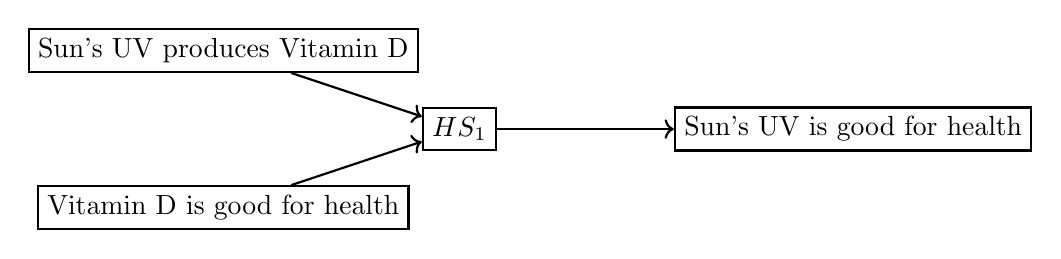
\begin{tikzpicture}
\tikzstyle{vertex} = [rectangle, draw = black, thick]
\tikzstyle{edge} = [->, thick]
\node[vertex] (p) at (0, 0) {Sun's UV produces Vitamin D};
\node[vertex] (HS) at (3, -1) {$HS_1$};
\node[vertex] (q) at (0, -2) {Vitamin D is good for health};
\node[vertex] (r) at (8, -1) {Sun's UV is good for health};
\draw[edge] (p)--(HS);
\draw[edge] (q)--(HS);
\draw[edge] (HS)--(r);
\end{tikzpicture}
\caption{Argument network using natural language} \label{argnet}
\end{figure}

% ARGUMENT NETWORK W/ REBUTTAL USING NATURAL LANGUAGE
\begin{figure}
\centering
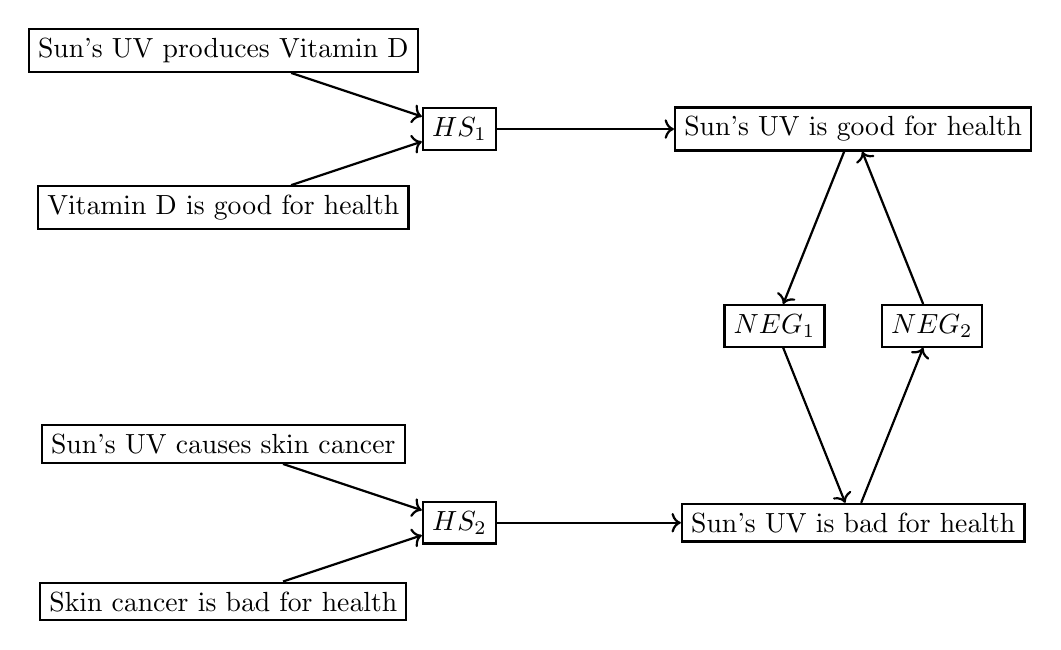
\begin{tikzpicture}
\tikzstyle{vertex} = [rectangle, draw = black, thick]
\tikzstyle{edge} = [->, thick]
% -----------------------------------
% Argument 1
\node[vertex] (p) at (0, 0) {Sun's UV produces Vitamin D};
\node[vertex] (HS1) at (3, -1) {$HS_1$};
\node[vertex] (q) at (0, -2) {Vitamin D is good for health};
\node[vertex] (r) at (8, -1) {Sun's UV is good for health};

\draw[edge] (p)--(HS1);
\draw[edge] (q)--(HS1);
\draw[edge] (HS1)--(r);

% -----------------------------------
% Argument 2
\node[vertex] (x) at (0, -5) {Sun's UV causes skin cancer};
\node[vertex] (HS2) at (3, -6) {$HS_2$};
\node[vertex] (y) at (0, -7) {Skin cancer is bad for health};
\node[vertex] (z) at (8, -6) {Sun's UV is bad for health};

\draw[edge] (x)--(HS2);
\draw[edge] (y)--(HS2);
\draw[edge] (HS2)--(z);
% -----------------------------------
% -----------------------------------
% CA-nodes
\node[vertex] (NEG1) at (7, -3.5) {$NEG_1$};
\node[vertex] (NEG2) at (9, -3.5) {$NEG_2$};

\draw[edge] (NEG1)--(z);
\draw[edge] (z)--(NEG2);
\draw[edge] (NEG2)--(r);
\draw[edge] (r)--(NEG1);
% -----------------------------------
\end{tikzpicture}
\caption{Argument network containing a rebuttal in natural language} \label{rebutargnet}
\end{figure}

\section{Conclusion}
In the article we've explored, the author describes the core concepts of argumentation in multiagent systems and formalizes the basic theory on arguments. He continues with discussing different protocols for argumentation, as well as explaining strategic argumentation with the help of fundamental game theory. The chapter ends with elaboration on the Argument Interchange Format, a standardized way of representing and exchanging arguments.

In our work on reviewing and commentating this chapter, we have provided minor contributions, in the form of examples given by us. We have also tried to rephrase various formal definitions to clear possible misunderstandings, or provide additional explanations to some parts of the material.
% ===================================================

\printbibliography[heading=bibintoc]
\end{document}
